\documentclass{article}

\usepackage{amsmath}
\usepackage{amsfonts}
\usepackage{amssymb}
\usepackage{graphicx}
\usepackage[dvipsnames]{xcolor}
\usepackage[margin=0.5in]{geometry}
\usepackage[hidelinks]{hyperref}
\usepackage{float}

\graphicspath{{.}{./img/}}

\usepackage{environ}
\NewEnviron{centerframebox}{\begin{center}\fbox{\parbox{0.92\textwidth}{\BODY}}\end{center}}

\title{Algorithms for Data Science \\ Exercise Sheet 1}
\author{
  Vladislav Imashev \\ \href{mailto:s05vimas@uni-bonn.de}{s05vimas@uni-bonn.de} \and
  \AA{AAAAAAAAAA AAAAAAA}{6} \\ \href{mailto:\AA{AAAAAAAAAAAAAAAAAAAA}{7}}{\AA{AAAAAAAAAAAAAAAAAAAA}{7}} \and
  German Mikhelson \\ \href{mailto:s17gmikh@uni-bonn.de}{s17gmikh@uni-bonn.de} \and
  Aleksandra Volynets \\ \href{mailto:s02avoly@uni-bonn.de}{s02avoly@uni-bonn.de} \and
  Nikita Morev \\ \href{mailto:s99nmore@uni-bonn.de}{s99nmore@uni-bonn.de}
}

\begin{document}
  \maketitle

  \setcounter{section}{1}
  \subsection{Number of Association Rules}
  \begin{centerframebox}
    Show that the number of all association rules over d items is $3^d - 2^{d+1} + 1$
    (see also, slide 22 of Lecture 2023-10-18).
  \end{centerframebox}
  Association rules take the form of $X \to Y$, where no item can be present in both $X$ and $Y$. $X$ can only be a subset that contains from $1$ to $d-1$ items (since we exclude the empty and the full set).
  For each of these subsets we must find a suitable $Y$ that is not empty and doesn't contain any items present in $X$.
  Let $n$ be the number of items in current subset $X$. Then $Y$ can contain from $1$ to $d-n$ items.
  The total number of subsets that can be $Y$ for a specific $X$ is: $2^{d-n} - 1$.
  Therefore, the total number of association rules can be calculated as follows:

  \begin{align*}
    &\sum_{n=1}^{d-1} {\left[\binom {d} {n}  \times \left({2} ^ {d-n} -1 \right) \right] = \sum_{n=0}^{d-1} {\left[\binom {d} {n} \times ( {2} ^ {d-n} -1) \right] - \left({2} ^ {d} -1 \right)}}  \\
    =& \sum_{n=0}^{d} {\left[\binom {d} {n} \times {2} ^ {d-n} \right] - \sum_{n=0}^{d} {\binom {d} {n} -} \left({2} ^ {d} -1 \right)} = {3} ^ {d} - {2} ^ {d} - {2} ^ {d} +1  \\
    =& {3} ^ {d} - {2} ^ {d +1} +1 \\
  \end{align*}

  \subsection{The Apriori Algorithm}
  \begin{centerframebox}
    A database has the following five transactions:

    \begin{center}
      \begin{tabular}{|c|c|}
        \hline
        TID & items bought \\ \hline
        1 & M, O, N, K, E, Y \\ \hline
        2 & D, O, N, K, E, Y \\ \hline
        3 & M, A, K, E \\ \hline
        4 & M, U, C, K, Y \\ \hline
        5 & C, O, K, E \\ \hline
      \end{tabular}
    \end{center}

    List all frequent itemsets with frequency threshold $t = 3$ (or equivalently, with
    a minimum support of $0.6$) by the Apriori algorithm. Give the details of your
    computation.
  \end{centerframebox}
  The given transaction database contains the following items $\mathcal{C}_1 = \{A,\, C,\, D,\, E,\, K,\, M,\, N,\, O,\, U,\, Y\}$.
  Out of them only $\mathcal{F}_1 = \{E,\, K,\, M,\, O,\, Y\}$ are frequent enough to pass our threshold.
  Because this is our first step, the candidate generation algorithm doesn't help much,
  and we have to compute the frequency of all $C^5_2 = 10$ combinations of two elements
  $\mathcal{C}_2 = \{EK,\, EM,\, EO,\, EY,\, KM,\, KO,\, KY,\, MO,\, MY,\, OY\}$.
  Here the frequencies are a bit harder to compute at a glance, but we eventually get
  $\mathcal{F}_2 = \{EK,\, EO,\, KM,\, KO,\, KY\}$.

  This time, for candidate generation we need to take all pairs of frequent itemsets starting with the same letter
  (or differing in only their last one) and combine them.
  We get the preliminary candidates $\{EKO,\, KMO,\, KMY,\, KOY\}$,
  but need to check if all their subsets are as also frequent, i. e. $\in \mathcal{F}_2$.
  The only itemset that passes this test is $\mathcal{C}_3 = \{EKO\}$, because neither $MO$, $MY$ or $OY$ are frequent.
  If we check the database, this itemset also happens to be frequent so $\mathcal{F}_3 = \{EKO\}$.

  Our final list of all frequent itemsets is as follows:
  $\{E,\, K,\, M,\, O,\, Y,\, EK,\, EO,\, KM,\, KO,\, KY,\, EKO\}$.

  \subsection{Correctness and Irredundancy of Apriori}
  \begin{centerframebox}
    Prove that the Apriori algorithm correctly and irredundantly generates all frequent itemsets.
    (First claim on slide 14 of Lecture 2023-10-25.)
  \end{centerframebox}
  \subsubsection{Correctness}
  %Prove that Apriori algorithm \\
  %1) generates all frequent itemsets \\
  %2) does not yield any infrequent one \\
  First, by induction on the length of the itemset $k$ show that the algorithm generates all frequent itemsets. \\
  \textbf{Basis:} all the frequent itemsets of the length $k = 1$ will be generated since on the first step we go through the set $S$ and leave frequent elements only (i.e. itemsets of the length 1). \\
  \textbf{Induction hypothesis:} assume that all the frequent itemsets of the length $k - 1, k > 1$ are generated by the Apriori algorithm.

  Prove that statement holds for an arbitrary frequent itemset $X$ of the length $k$.
  Let $X = x_1 x_2 ... x_k$. Hence, we could consider:
  $$X_1 = x_1 x_2 ... x_{k-2} x_{k-1}$$
  $$X_2 = x_1 x_2 ... x_{k-2} x_k$$

  Since $X_1, X_2 \subset X$ and $X$ is frequent, $X_1$ and $X_2$ are also frequent. Moreover, $X_1$ and $X_2$ have the length $k-1$, hence they are generated by the Apriori algorithm according to the induction hypothesis. This means that $X_1,\, X_2 \in F_{k-1}.$ Having this, we can argue that $X$ will be generated as the concatenation of the common $(k-2)$-prefix of $X_1$ and $X_2$, $x_{k-1}$ and $x_k$, so $X$ will be in the set of candidates of the length $k$. And therefore $X$ will surely get to the set $F_k$ since $X$ is frequent and this implies that all its subsets are frequent too. Hence, $X$ is generated by the algorithm.

  Second, prove that none of the infrequent itemsets will be generated. On each iteration of the algorithm, we compare the frequency of the generated candidates with the threshold. Therefore, infrequent candidates will not get to the $F$ set and therefore infrequent candidates will not be generated.

  \subsubsection{Irredundancy}

  By induction on the length of the itemset $k$ show that there are no two identical frequent itemsets generated by the algorithm. \\
  \textbf{Basis:} all the generated frequent itemsets of the length $k = 1$ will be different since there is no two identical elements in the set S. \\
  \textbf{Induction hypothesis:} assume that there are no two identical frequent itemsets of the length $k - 1, k > 1$. In other words, there are no two identical itemsets in the $F_{k-1}$.

  Prove that statement holds for $F_k$. Consider the set of the candidates $C_k$. According to the induction hypothesis, all the itemsets in the set $F_{k-1}$ are different. We generate the set of candidates $C_k$ as a concatenation of the common $(k-2)$-prefix of the itemsets from $F_{k-1}$ and their last two elements. Hence, these last two elements are always different (otherwise, there would be a pair of identical itemsets in $F_{k-1}$). Hence, there are no two identical itemsets if the $C_k$. The set $F_{k}$ is a subset of $C_k$, therefore all the elements in $F_{k}$ are surely different.

  \subsection{Complexity of Apriori}
  \begin{centerframebox}
    Prove that the Apriori algorithm generates the set of frequent itemsets in incremental polynomial time.
    (Second claim on slide 14 of Lecture 2023-10-25.)
  \end{centerframebox}
  Consider the set: $S = \{s_{1}, ... , s_{n}\}$. There is an algorithm that prints $s_{\pi(i)}$. And between $s_{\pi(i-1)}$ and $s_{\pi(i)}$ we have time $t_{i}$, which is limited by the following polynomial:
  $$t_{i} \leq P(|Input| + |s_{\pi(1)}| + ... + |s_{\pi(i)}|)$$

  In our task, the power of the inputs is $|Input| = |D| + |S|$. Define $|Input| = m$.\\

  To obtain a general assessment of the Apriori algorithm performance, let's evaluate each of its components and add:

  \textbf{1.} $F_{i} = \{x \in C_{i}: |D[x]| \geq t\}$, where $t$ is threshold. \\
  So, to compose the set $F_{i}$ we need:
  $$O(F_{i}) = O(|C_{i}| \cdot |D|)$$

  Let's continue our assessment:
  $$O(F_{i}) = O(|C_{i}| \cdot |D|) \leq O(|F_{i-1}| \cdot |Input|)$$

  Let's evaluate $|F_{i-1}|$. Let's calculate the number of operations to compose $F_{i}$. Let's consider the worst case, when all our chains have the same prefix, i.e. $i-1$ elements are the same and differ in only one element. In this case, the total possible combinations of chains for $F_{i}$ will be $|F_{i-1}|^2 - |F_{i-1}|$, remove the number of chains that did not form a chain of length $i$. Those the number of operations is limited by a 2nd degree polynomial. This means we can limit this value by a polynomial with an input of size $F_{i-1}$:
  $$|F_{i}| \leq T(|F_{i-1}|),$$ $T$ is a polynomial.

  And the final product is a polynomial, so we get:
  $$O(F_{i}) = O(|C_{i}| \cdot |D|) \leq O(|F_{i-1}| \cdot |Input|) \leq O(T(|F_{i-2}|) \cdot m) \leq O(R),$$ where $R$ is a polynomial.

  \textbf{2.} $print$ $F_{i}$ \\
  The number of operations we need to print all the elements from $F_{i}$ is $|F_{i}|$, which we can evaluate as a polynomial $L$, as written above.\\

  \textbf{3.} $C_{i+1} := CandidateGeneration(F_{i})$ \\
  This method consists of several stages, which we will evaluate separately:

  1) We can make up the number of pairs $X, Y \in F_{i}$ with the following number:
  $$O \left( \binom {2} {|F_{i}|}\right) = O\left(\frac{|F_{i}| \cdot |F_{i-1}|}{2}\right) \leq O(|F_{i}|^2) \leq J(|F_{i-1}|),$$ where $J$ is a polynomial.

  2) The next step is to find out the number of different elements in the sets $X$ and $Y$. Thus, checking the occurrence of elements $X$ in $Y$ is evaluated in the following way:
  $$O(|X| \cdot |Y|) = O(i^2),$$
  because we work with subsets containing chains of length $= i$. \\
  Note that $1 \leq |Input|, 1 \leq |F_{1}|, ... , 1 \leq |F_{i-1}|$, hence $i \leq |Input| + |F_{1}| + ... + |F_{i-1}|$, hence
  $$O(i^2) \leq O(P(|Input| + |F_{1}| + ... + |F_{i-1}|)),$$ where $P$ is a polynomial.

  3) The number of operations to obtain a new candidate by combining the sets $X$ and $Y$ can be roughly estimated as $i^2$, which, in turn, is estimated by a polynomial, as in the previous paragraph.\\

  4) And the last action is that the resulting set of candidates contains subsets $Z_{k} \in F_{i}$. Accordingly, to check all $Z_{k}$ from $Z$ we will need the following number of operations, which we will immediately estimate:
  $$O\left(\binom {i} {i + 1}\right) \cdot |F_{i}| = O((i + 1) \cdot |F_{i}|) \leq O((Q + 1) \cdot Q) \leq O(2Q^2),$$ where $Q$ is a polynomial.
  Let's add up all the estimates to estimate the complexity of the algorithm:
  $$O(C_{i+1}) \leq O(J^2 \cdot (P + M + 2Q^2)) = O(U)$$
  Finally, having obtained estimates for all components of the original algorithm, we estimate the complexity of the Apriori algorithm:
  $$O(\text{Apriori algorithm}) \leq O(R) + O(L) + O(U) \leq O(E)$$
  Thus, the complexity of the entire algorithm is limited by a polynomial.

  \subsection{Rule Generation}
  \begin{centerframebox}
    For the transaction database given in Task 2 above list all association rules with
    a minimum support of $0.6$ and minimum confidence of $0.8$. Use the algorithm
    given on Slides 17--18 of Lecture 2023-10-25.
  \end{centerframebox}

  \begin{figure}[H]
    \centering
    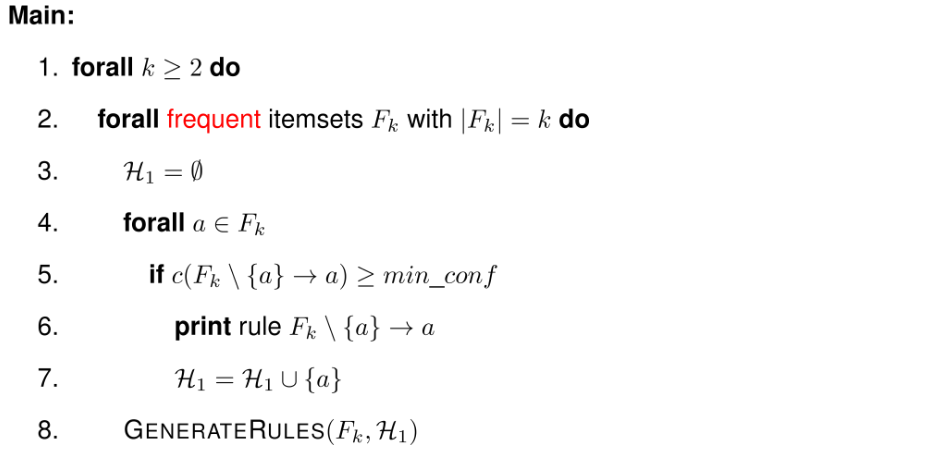
\includegraphics[width=15cm, height=7.5cm]{Rule generation 1.png}
    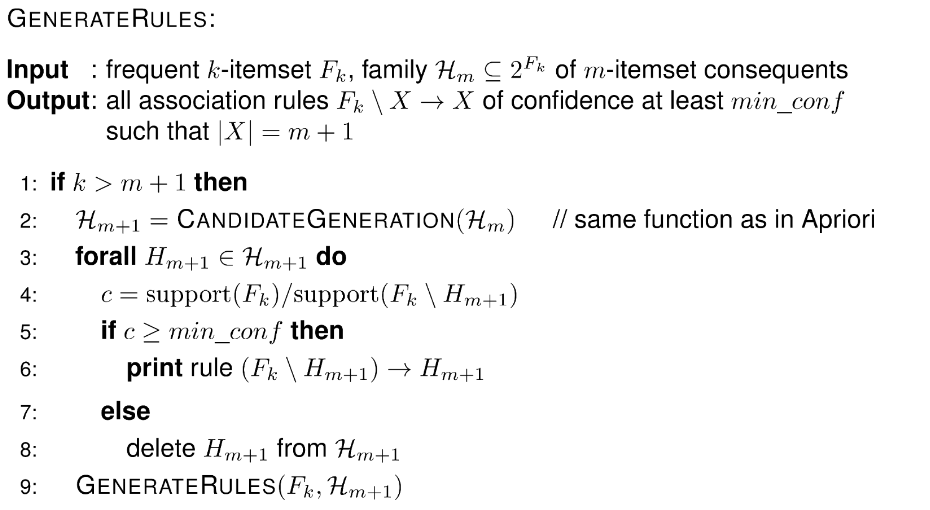
\includegraphics[width=15cm, height=8.3cm]{Rule generation 2.png}
    \caption{The algorithm for rules generation}
    \label{fig:enter-label}
  \end{figure}

  Following the algorithm, first we consider all possible rules of size $k=2$ from the set of frequent k-itemsets $\mathcal{F}_2 = \{\{E,K\},\, \{E,O\},\, \{K,M\},\, \{K,O\},\, \{K,Y\}\}$, which already satisfies our minimum support criteria.

  Calculation example:
  $${F}_k = \{E, O\}$$
  $$c({F}_k \setminus \{E\} \to E) = c(O \to E) = \dfrac{|D[\{E, O\}]|}{|D[\{O\}]|} = \dfrac{3}{3} = 1$$
  $$c({F}_k \setminus \{O\} \to O) = c(E \to O) = \dfrac{|D[\{E, O\}]|}{|D[\{E\}]|} = \dfrac{3}{4} = 0.75$$

  \begin{center}
    \begin{tabular}{|l|r|}
      \hline
      \textbf{rule} & \textbf{confidence} \\ \hline
      E $\to$ O & \textcolor{BrickRed}  {$0.75$} \\ \hline
      O $\to$ E & \textcolor{OliveGreen}{$1   $} \\ \hline
      E $\to$ K & \textcolor{OliveGreen}{$1   $} \\ \hline
      K $\to$ E & \textcolor{OliveGreen}{$0.8 $} \\ \hline
      O $\to$ K & \textcolor{OliveGreen}{$1   $} \\ \hline
      K $\to$ O & \textcolor{BrickRed}  {$0.6 $} \\ \hline
      M $\to$ K & \textcolor{OliveGreen}{$1   $} \\ \hline
      K $\to$ M & \textcolor{BrickRed}  {$0.6 $} \\ \hline
      K $\to$ Y & \textcolor{BrickRed}  {$0.6 $} \\ \hline
      Y $\to$ K & \textcolor{OliveGreen}{$1   $} \\ \hline
      \end{tabular}
  \end{center}

  $$\mathcal{H}_1 = \{\{E\}, \{K\}\}$$

  We cannot generate more rules, because $k \ngtr m + 1$, where $k=2$ and $m=1$. \\

  Then we consider all rules with a single item from the set of frequent 3-itemsets $\mathcal{F}_3 = \{E,K,O\}$.
  \begin{center}
    \begin{tabular}{|l|r|}
      \hline
      \textbf{rule} & \textbf{confidence} \\ \hline
      E,O $\to$ K & \textcolor{OliveGreen}{$1   $} \\ \hline
      E,K $\to$ O & \textcolor{BrickRed}  {$0.75$} \\ \hline
      K,O $\to$ E & \textcolor{OliveGreen}{$1   $} \\ \hline
      \end{tabular}
  \end{center}

  $$\mathcal{H}_1 = \{\{E\}, \{K\}\}$$

  We can continue generating more rules. First we generate new candidates:
  $$\mathcal{H}_2 = \{E, K\}$$

  And finally we consider all rules of size $k=3$ with our new candidates. \\

  Calculation example:
  $$c({F}_k \setminus \{E,K\} \to \{E,K\}) = c(O \to E,K) = \dfrac{|D[\{E, K, O\}]|}{|D[\{O\}]|} = \dfrac{3}{3} = 1$$

  \begin{center}
    \begin{tabular}{|l|r|}
      \hline
      \textbf{rule} & \textbf{confidence} \\ \hline
      O $\to$ E,K & \textcolor{OliveGreen}{$1   $} \\ \hline
      \end{tabular}
  \end{center}

  We cannot generate more rules, because $k \ngtr m + 1$, where $k=3$ and $m=2$. \\

  The final list of all association rules with
  a minimum support of $0.6$ and minimum confidence of $0.8$:
  \begin{center}
      O $\to$ E \\
      E $\to$ K \\
      K $\to$ E \\
      O $\to$ K \\
      M $\to$ K \\
      Y $\to$ K \\
      E,O $\to$ K \\
      K,O $\to$ E \\
      O $\to$ E,K \\
  \end{center}
\end{document}
